%label:"exm:sphereRotation"
%type:"example"
%name:"rotation of Sphere"


    Consider $S^2=\{(x_0, x_1, x_2)\;|\;x_0^2+x_1^2+x_2^2=1\}$  equipped with the symplectic form agreeing with the standard metric induced from $\RR^3$.
    Take the Hamiltonian 
    \begin{align*}
        H:S^2\to&\RR\\
        (x_0,x_1,x_2)\mapsto& x_2
    \end{align*}
    as drawn in \cref{fig:hamiltonianOnSphere}.
    Since Hamiltonian flow preserves the level sets of $H$, we know that the latitudinal slices are orbits under the action of the Hamiltonian flow. 
    To show that the Hamiltonian flow uniformly rotates the sphere, consider the map  $\phi:S^2\setminus\{(0,0,1), (0,0,-1)\}\into S^1\times \RR\subset \RR^3$, where $S^1\times \RR=\{(x_0, x_1, x_2)\;|\; x_0^2+x_1^2=1\}$, and the embedding is given by the latitudinal projection.
    This projection (the \emph{Gall-Peters} map projection) is area-preserving, and so $\phi$ is a symplectic embedding.
    In these new coordinates, $\omega=d\theta\wedge dx_2$ and $H=x_2$. In the Gall-Peters' coordinates,   $V_H=\partial_\theta$. 
    %tag:000X
%label:"fig:hamiltonianOnSphere"
%author:JeffHicks
%name:"rotation of sphere"
%type:"figure"
%parent:exm:sphereRotation
%caption:"The Hamiltonian flow of the standard height function rotates the sphere counterclockwise relative to the north pole"

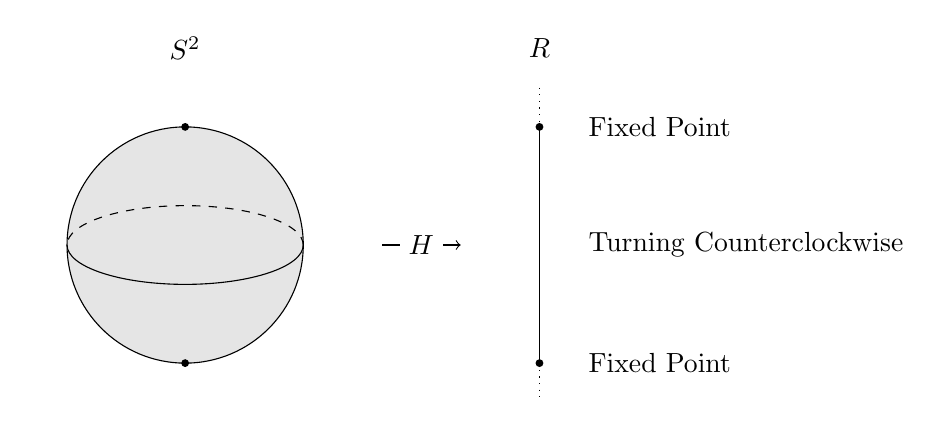
\begin{tikzpicture}
    \draw[fill=gray!20]  (-2,2) ellipse (1.5 and 1.5);
    \begin{scope}[]
    \clip  (-4,2) rectangle (0,3);
    \draw[dashed]  (-2,2) ellipse (1.5 and 0.5);
    \end{scope}
    \begin{scope}[]
    \clip  (-4,2) rectangle (0,1);
    \draw  (-2,2) ellipse (1.5 and 0.5);
    \end{scope}
    
    \draw (2.5,3.5) -- (2.5,0.5);
    \draw[->] (0.5,2) -- (1.5,2);
    \node[fill=white] at (1,2) {$H$};
    \draw[dotted] (2.5,4) -- (2.5,3.5) (2.5,0.5) -- (2.5,0);
    \node at (-2,4.5) {$S^2$};
    \node at (2.5,4.5) {$\mathbb R$};
    \node[right] at (3,3.5) {Fixed Point};
    \node[right] at (3,2) {Turning Counterclockwise};
    \node[right] at (3,0.5) {Fixed Point};
    \node[circle, fill=black, scale=.3] at (-2,3.5) {};
    \node[circle, fill=black, scale=.3] at (-2,0.5) {};
    \node[circle, fill=black, scale=.3] at (2.5,0.5) {};
    \node[circle, fill=black, scale=.3] at (2.5,3.5) {};
    \end{tikzpicture}

